\documentclass[a4paper,12pt]{article}
\usepackage[margin=1in,headheight=15pt,headsep=6mm,footskip=9mm]{geometry}
\usepackage[T1]{fontenc}
\usepackage{lmodern}
\usepackage{amsmath,amssymb,booktabs,array,tabularx}
\usepackage{graphicx,wrapfig,needspace}
\usepackage{tikz}
\usetikzlibrary{arrows.meta,calc}
\usepackage{caption,fancyhdr,microtype}
\usepackage[colorlinks=true,linkcolor=black,urlcolor=blue!50!black]{hyperref}
\hypersetup{pdftitle={CuRo6R -- Kinematic modelling},pdfsubject={Project 1F: kinematic models, Jacobians and analytical inverse kinematics}}
\definecolor{dhink}{HTML}{243747}
\definecolor{dhblue}{HTML}{2164A1}
\definecolor{dhred}{HTML}{B84338}
\definecolor{dhgreen}{HTML}{337A55}
\definecolor{dhgold}{HTML}{A66816}
\definecolor{dhpurple}{HTML}{79509A}
\definecolor{dhgray}{HTML}{78838C}
\pagestyle{fancy}
\fancyhf{}
\fancyhead[L]{\small\sffamily Kinematics-Grounded Motion Planning for Robots}
\fancyhead[R]{\small\sffamily Project 1F \enspace |\enspace CuRo6R}
\fancyfoot[C]{\small\thepage}
\renewcommand{\headrulewidth}{0.3pt}
\setlength{\parindent}{0pt}
\setlength{\parskip}{3pt}
\AtBeginDocument{%
  \setlength{\abovedisplayskip}{8pt plus 2pt minus 3pt}%
  \setlength{\belowdisplayskip}{8pt plus 2pt minus 3pt}%
  \setlength{\abovedisplayshortskip}{0pt plus 2pt}%
  \setlength{\belowdisplayshortskip}{5pt plus 2pt minus 2pt}%
}
\captionsetup{font=small,labelfont=bf}
\newcommand{\frameid}[1]{\{#1\}}
\newcommand{\jointid}[1]{\mathrm{J}_{#1}}
\newcommand{\vect}[1]{\boldsymbol{#1}}
\newcommand{\trans}{\mathsf T}
\newcommand{\ex}{\vect{e}_x}
\newcommand{\ez}{\vect{e}_z}
\newcommand{\qq}{\vect{q}}
\newcommand{\Rcal}{\mathcal R}
\newcommand{\DHDiagram}[1]{%
  \resizebox{\linewidth}{!}{\input{figures/dh_step_#1.tex}}%
}
\newcommand{\DHPanel}[4]{%
  \begin{minipage}[t]{0.486\linewidth}
    {\small\sffamily\bfseries\color{dhink}#1}\par\vspace{1pt}
    {\small #2}\par\vspace{1pt}
    \centering\DHDiagram{#3}\par
    \raggedright\small #4
  \end{minipage}%
}
\begin{document}
\section{Forward kinematics models}
\label{sec:fk-models}
\providecommand{\DHSectionFile}{sections/dh_parameters.tex}
\input{\DHSectionFile}
\providecommand{\PoESectionFile}{sections/poe_model.tex}
\input{\PoESectionFile}
\providecommand{\FKVerificationFile}{sections/fk_verification.tex}
\input{\FKVerificationFile}
\providecommand{\JacobianSectionFile}{sections/jacobian.tex}
\input{\JacobianSectionFile}
\providecommand{\AnalyticalIKSectionFile}{sections/analytical_ik.tex}
\input{\AnalyticalIKSectionFile}

\section{Connectivity analysis}
\label{sec:connectivity}
In this section we provide a qualitative analysis of the conditions required for a non-singular
change of solutions, and the sequence of steps we used to numerically get a trajectory for a
nonsingular change of solution with constant tool orientation.

\begin{figure}[!ht]
\centering
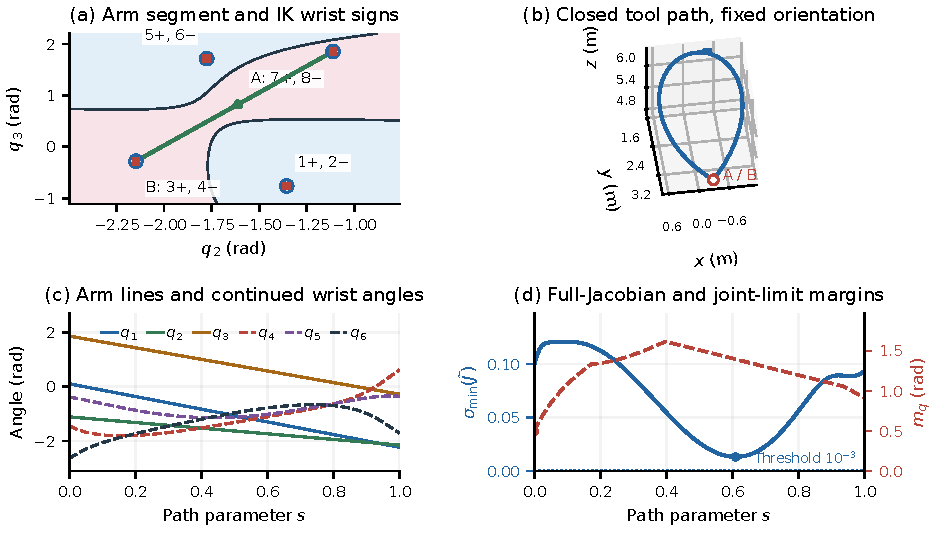
\includegraphics[width=\linewidth]{figures/connectivity_linear.pdf}
\caption{Arm singularities and a fixed-orientation solution change
in (a) joint space and (b) the wrist-centre workspace,
with $\rho_w=\sqrt{x_w^2+y_w^2}$.
The cusps indicate that the CuRo6R's positioning chain is cuspidal: it can
change between IK solutions without crossing an arm singularity.
At the marked target, $t_1<t_2<t_3<t_4$.
The folds $F_{ij}$ merge $t_i,t_j$; cusps $C_k$ are indexed by the
root $k$ shared by their incident folds, with $u/r$ superscript distinguishing upper/right.}
\label{fig:arm-singularity-map}
\label{fig:connectivity-linear}
\end{figure}

\textbf{A straight arm path with fixed tool orientation.} We index each full configuration $\vect{q}^{(i)}$ by its arm root $t_i$
on the chosen wrist branch. We choose the initial joint configuration
$\vect{q}^{(4)}=(0.1024,\allowbreak-1.1124,\allowbreak1.8547,\allowbreak-1.4399,\allowbreak-0.3835,\allowbreak-2.6486)^\trans$
(in radians), compute ${}^0T_{E,d}=\operatorname{FK}(\vect{q}^{(4)})$, and solve the IK
for this pose, obtaining eight solutions. Excluding the initial solution,
exactly one has the same signs of $\det J_{v,\mathrm{arm}}$ and $\sin q_5$:
$\vect{q}^{(2)}\approx(-2.2287,\allowbreak-2.1482,\allowbreak-0.2788,\allowbreak0.6181,\allowbreak-0.3524,\allowbreak-1.7072)^\trans$.
This candidate also satisfies the endpoint joint-limit and singularity
margins, but matching signs alone does not guarantee a nonsingular connection.

We discretize the straight path between their arm joints
$\vect{q}_a=(q_1,q_2,q_3)^\trans$:
\begin{equation}
 \vect{q}_a(s)=(1-s)\vect{q}_a^{(4)}+s\vect{q}_a^{(2)},\qquad 0\leq s\leq1,
 \label{eq:connectivity-arm-segment}
\end{equation}
where $s$ measures path advancement. At each sample, we remove the arm
orientation from the desired orientation ${}^0R_{E,d}$ by computing
${}^3R_{E,d}(s)=({}^0R_3(\vect{q}_a(s)))^\trans\,{}^0R_{E,d}$.
We recover the wrist angles using \eqref{eq:ik-wrist-solutions}, preserving
the initial sign of $\sin q_5$ and choosing continuous angle representatives.
The tool orientation remains fixed while its position is free to vary.

We continue only while joint-limit clearance is nonnegative, the arm
determinant retains its sign, $|\sin q_5|>10^{-6}$, and
$\sigma_{\min}(\widetilde J)>10^{-3}$, where
$\widetilde J=\operatorname{diag}(\ell_c^{-1}I_3,I_3)\,{}^0J_E$
uses the characteristic length $\ell_c=2\,\mathrm m$ to scale the linear
velocity rows. A failed check stops the attempt; acceptance also requires
reaching the selected goal. Figure~\ref{fig:connectivity-linear} shows the
accepted change from $\vect{q}^{(4)}$ to $\vect{q}^{(2)}$. These checks concern the sampled
configurations, so a finer discretization improves confidence of real success.


\clearpage
\appendix
\section{DH frame constructions}
\label{app:dh-constructions}

Figure~\ref{fig:dh-steps} collects all six frame-to-frame constructions at the
home configuration ($\vect{q}=\vect{0}$), using one fixed viewing direction and length scale.
Lengths are in metres; angles are shown in degrees for readability.

\begingroup
\captionsetup{hypcap=false}
\centering
\DHPanel{1\quad Base to shoulder: $\frameid{0}\to\frameid{1}$}
 {$d_1=1,\quad\theta_1=q_1,\quad\alpha_1=-60^\circ,\quad a_1=0.8$}{1}
 {The full base height is $1$ m. The $30^\circ$ URDF roll of joint 2 gives
 $\alpha_1=30^\circ-90^\circ=-60^\circ$.}
\hfill
\DHPanel{2\quad Shoulder to elbow: $\frameid{1}\to\frameid{2}$}
 {$d_2=1.25,\quad\theta_2=q_2,\quad\alpha_2=90^\circ,\quad a_2=2$}{2}
 {The $x$ axes remain parallel. The offset along $z_1$ and the common normal
 along $x_2$ locate $O_2$ on joint 3.}

\vspace{10pt}
\DHPanel{3\quad Axis intersection: $\frameid{2}\to\frameid{3}$}
 {$d_3=0.75,\quad\theta_3=q_3+90^\circ,\quad\alpha_3=90^\circ,\quad a_3=0$}{3}
 {$O_3$ is the intersection of the extended axes. Choosing $x_3=y_2$
 explains the fixed $+90^\circ$ offset in $\theta_3$.}
\hfill
\DHPanel{4\quad Reach the wrist: $\frameid{3}\to\frameid{4}$}
 {$d_4=2.5,\quad\theta_4=q_4,\quad\alpha_4=-90^\circ,\quad a_4=0$}{4}
 {The distance starts at $O_3$, rather than the joint-4 cylinder.
 The two physical offsets add: $d_4=1.5+1$.}

\vspace{10pt}
\begin{minipage}{\linewidth}
\DHPanel{5\quad Coincident origins: $\frameid{4}\to\frameid{5}$}
 {$d_5=0,\quad\theta_5=q_5,\quad\alpha_5=90^\circ,\quad a_5=0$}{5}
 {The origins coincide, although the joint centres do not.
 Here $x_4=x_5$ and the extended joint-6 axis passes through the wrist centre.}
\hfill
\DHPanel{6\quad Wrist to endpoint: $\frameid{5}\to\frameid{6}$}
 {$d_6=1.5,\quad\theta_6=q_6,\quad\alpha_6=0,\quad a_6=0$}{6}
 {At home the two frames have parallel axes. $O_6=O_E$;
 the fixed endpoint alignment changes orientation only.}

\vspace{9pt}
\captionof{figure}{Standard DH frame assignment. Cylinders denote physical revolute joints
 $\jointid{i}$; dots mark DH origins $O_i$.
 \textcolor{dhred}{$x$}, \textcolor{dhgreen}{$y$} and \textcolor{dhblue}{$z$}
 axes retain their colours. Dashed lines extend joint axes;
gold dimensions locate the origins. Boxed angle sketches show the rotation $x_2\to x_3$ about $+z_2$,
 giving $\theta_3^0$, and the signed twist
 $z_{i-1}\to z_i$ about $+x_i$ (with the first direction translated to the same
 point). Cylinder orientation, size and viewing direction are reused between panels;
 drawings are schematic.}
\label{fig:dh-steps}
\end{minipage}
\par\endgroup

\end{document}
